\documentclass[conference]{IEEEtran}
\IEEEoverridecommandlockouts

\usepackage{cite}
\usepackage{amsmath,amssymb,amsfonts}
\usepackage{mathrsfs}
\usepackage{subfigure}
\usepackage{booktabs}
\usepackage{yhmath}
\usepackage{enumitem}
\usepackage{amsthm}
\usepackage{float}
\usepackage{graphicx}
\usepackage{textcomp}
\usepackage{xcolor}
\usepackage{marvosym}
\usepackage{algorithm}
\usepackage{algorithmic}
\renewcommand{\algorithmicrequire}{ \textbf{Input~~:}}
\renewcommand{\algorithmicensure}{ \textbf{Output:}} 
\def\BibTeX{{\rm B\kern-.05em{\sc i\kern-.025em b}\kern-.08em
T\kern-.1667em\lower.7ex\hbox{E}\kern-.125emX}}
\usepackage{fancyhdr}
\usepackage{bm}
\usepackage[top=2cm, bottom=2cm, left=2cm, right=2cm]{geometry}
\newtheorem{definition}{Definition}
\newtheorem{theorem}{Theorem}
\newtheorem{assumption}{Assumption}
\newtheorem{lemma}{Lemma}
\newtheorem{problem}{Problem}
\newtheorem{remark}[theorem]{Remark}

\title{Appendices}

\begin{document}
\begin{appendices}
\section{The derivation of QBER}
Quantum Bit Error Rate (QBER) refers to the bit-flip error caused by the collapse decoherence here. First, we provide a theorem:
\begin{theorem}
\label{QBER}
Given the collapse decoherence model with the entanglement fidelity $F(\left| {{\psi}} \right\rangle _d^f) $, its QBER is deduced as $p'' = F^{-1}(F^d_{p''}, d)$.
\end{theorem}
\begin{proof}
The quality of each link-level entanglement is compromised to varying degrees due to the bit-flip errors caused by the collapse decoherence noise model. Therefore, the QBER of each link-level entanglement transmission is determined by the entanglement quality. In our works, the link-level entanglement fidelity is used to evaluate the entanglement quality, and denoted as
\begin{equation}
\begin{aligned}
	F(\left| {{\psi}} \right\rangle _d^f) = {\sqrt {fd}} p{(1 - p)^{f \cdot d - 1}} {e^{ - \tau {{(\Delta x)}^2}}},
\end{aligned}
\end{equation}
It is determined by the entanglement dimension $d$, measured probability $p$, and the entanglement link length $\Delta x$ with the assumption of $f=1$.

For two-qubit entanglement, Zhao \textit{et al.} \cite{zhao2022e2e} introduce an equation to describe the relationship between the QBER and the fidelity:
\begin{equation}
	\begin{aligned}
		F = p''^2 + (1-p'')^2.
	\end{aligned}
\end{equation}
It is derived from the flipping and no-flipping simultaneously occurring on both two qubits, which maintains identical two-qubit entanglement state, i.e., the fidelity indicates the degree to which quantum states remain stable.

\begin{figure}[h]
	\centering
	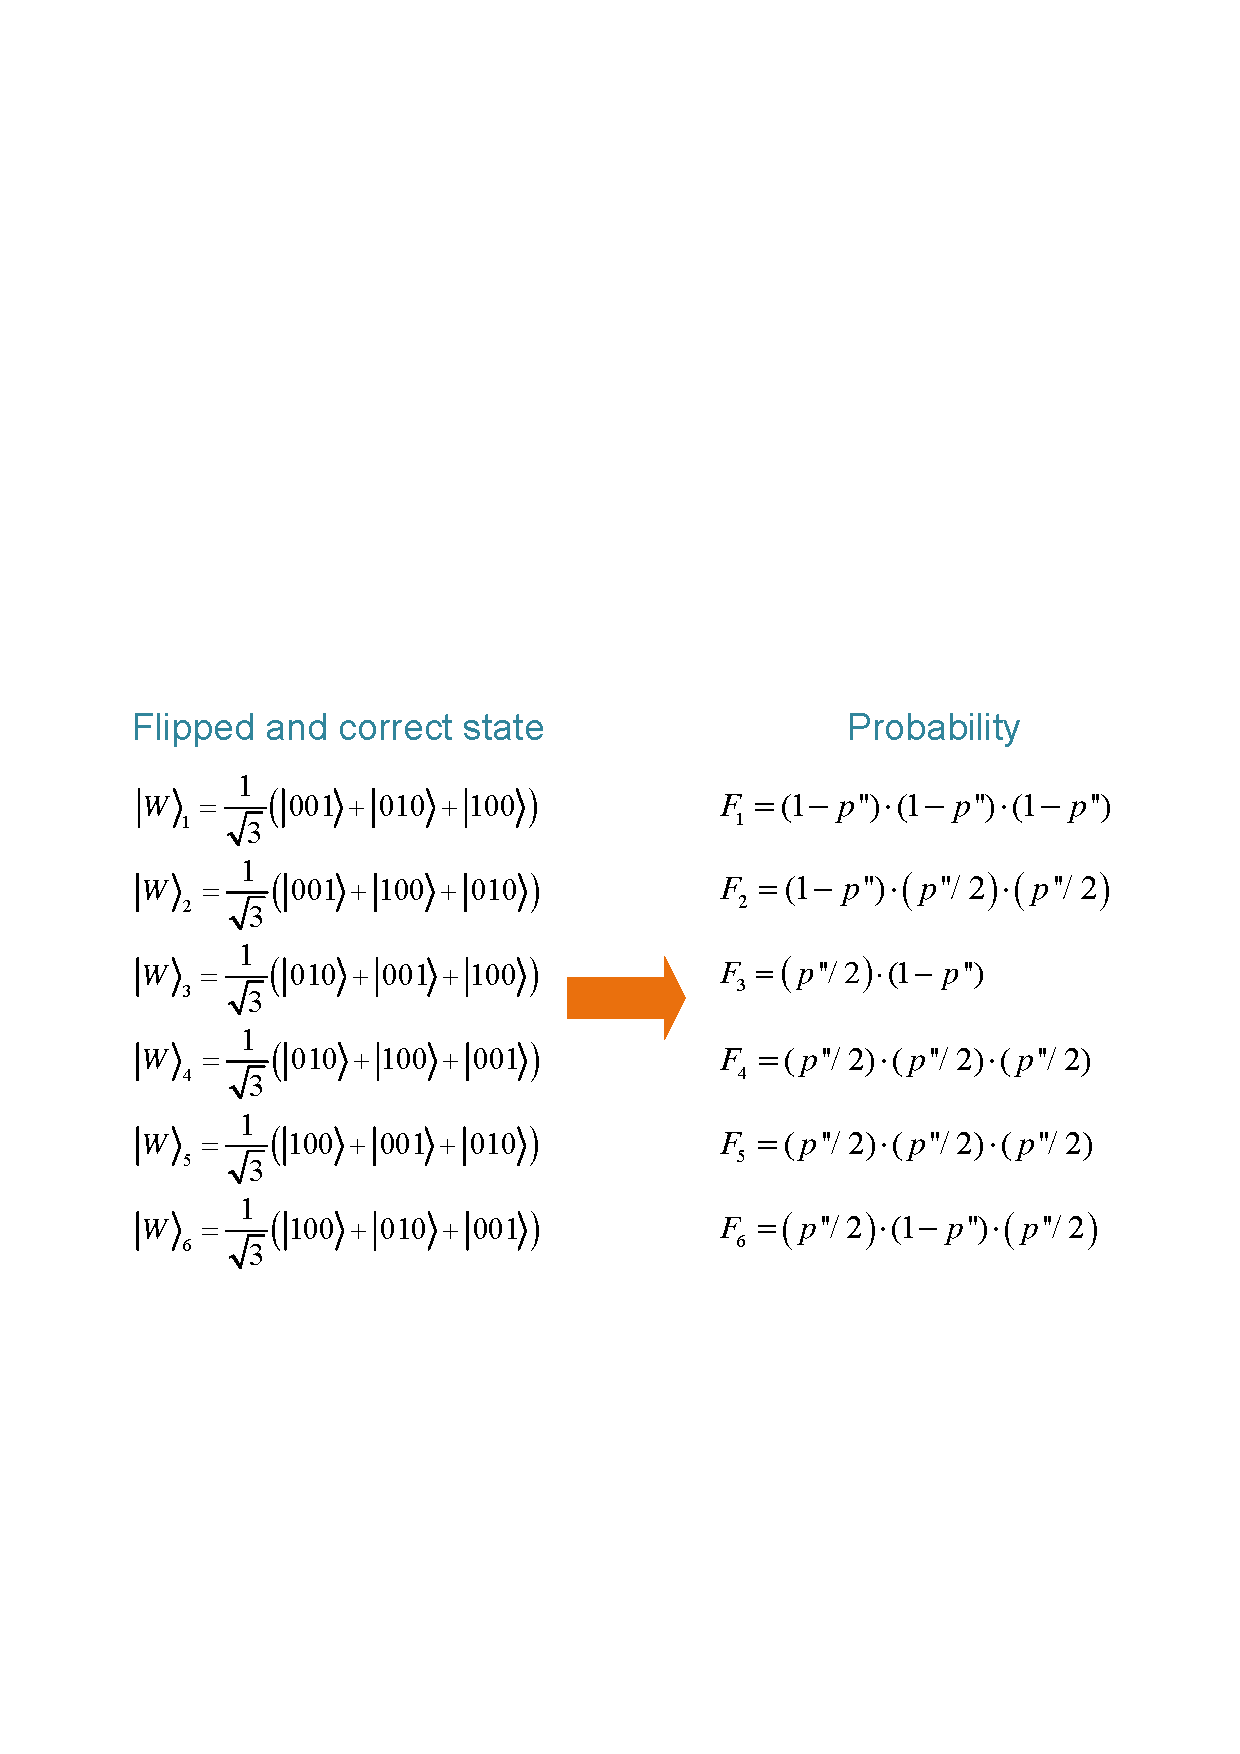
\includegraphics[width=0.9\linewidth]{images/three-qubit-entanglement.pdf}
	\caption{A three-qubit W entanglement state.}
	\label{three-qubit-entanglement}
\end{figure}

It is completely different under the scheme of the multi-qubit entanglement. As is shown in Fig.~\ref{three-qubit-entanglement}, a three-qubit entanglement is written as \textit{W} state as $\left| W \right\rangle  = \frac{1}{{\sqrt 3 }}(\left| {001} \right\rangle  + \left| {010} \right\rangle  + \left| {100} \right\rangle )$. If the first qubit in the $1$-dimension state $\left| {001} \right\rangle$ flips from $\left | 0 \right \rangle$ to $\left | 1 \right \rangle$, the state in $1$-dimension changes from $\left| {001} \right\rangle$ to $\left| {100} \right\rangle$ according to the rules of \textit{W} state which indicates only one qubit can be at state $\left | 1 \right \rangle$ in a dimension. For a $3$-dimensional entanglement state, there are totally $3!=6$ bit-flip results that can maintain the original results, i.e., $\left| W \right\rangle  = \left| {{W_i}} \right\rangle ,i = 1,2,...,6$. Fig.~\ref{three-qubit-entanglement} provides the fidelity of each bit-flip result. Hence, the total fidelity of $\left| W \right\rangle$ is denoted as $F^3 = \sum\limits_{i = 1}^{3!} {{F^3_i}}$. It is a misalignment problem in the square matrix. And so forth, the fidelity of $d$-dimensional entanglement is derived as:
\begin{equation}
	\begin{aligned}
		{F^d_{p''}} = & C_d^d{(1 - p'')^d} + \\
		&\sum\limits_{k = 2}^d {\left[ {C_d^{d - k}\left( {k!\sum\limits_{kk = 0}^k {\frac{{{{( - 1)}^{kk}}}}{{kk!}}} } \right){{(1 - p'')}^{d - k}}{{(p''/2)}^k}} \right]}.
	\end{aligned}
\end{equation}

Given a dimension number $d$ and a link-level fidelity $F^d$, we can obtain the QBER $p''$ of this entanglement link by the inverse function $F^{-1}$ of $F^d$. Further, we can obtain the average QBER of an E2E entanglement route for a request.
\end{proof}

\section{The derivation of QBER}
The phase flip is a specific error in the quantum state, which has no equivalent in classical computing like the bit-flip error. Whereas a bit flip swaps the probabilities of a qubit being $\left | 0 \right \rangle$ or $\left | 1 \right \rangle$, a phase flip swaps the probabilities of the qubit being $+$ or $-$, i.e., the direction of the particle rotation. First, we provide a theorem:
\begin{theorem}
\label{QPER}
Given the collapse decoherence model with the entanglement fidelity $F(\left| {{\psi}} \right\rangle _d^f) $, its QPER is deduced as $p' = F^{-1}(F^d_{p'}, d)$.
\end{theorem}
\begin{proof}
Assume a QPER for a two-qubit entanglement is denoted by $p'$, its fidelity can be deduced by $F^2=p'^2+(1-p')^2$ because $\left| W \right\rangle  = \frac{1}{{\sqrt 2 }}(+ \left| {01} \right\rangle  + \left| {10} \right\rangle )$ is oppositely same as $\left| W \right\rangle  = \frac{1}{{\sqrt 2 }}(- \left| {01} \right\rangle  - \left| {10} \right\rangle )$. That two phases both flip is equal in that there is no flipping for entanglement state $\left| W \right\rangle$. Likewise, for the three-qubit link-level entanglement, it fidelity is $F^3 = p'^3+(1-p')^3$. Further, the fidelity of $d$-dimensional link-level entanglement is 
\begin{equation}
	F^d = p'^d+(1-p')^d.
\end{equation}

From our introduced collapse decoherence model $F(\left| {{\psi}} \right\rangle _d^f) = \sqrt {fd} p{(1 - p)^{f \cdot d - 1}} {e^{ - \tau {{(\Delta x)}^2}}}$, we can obtain a QPER $p'$ of a link-level $d$-dimensional entanglement solved by the inverse function $F^{-1}(F^d_{p'}, d)$.
\end{proof}

We can see that, QBER is the same as QPER for a link-level entanglement in the two-qubit transmission scheme due to the same fidelity formulation $F^2=p^2+(1-p)^2$.

\end{appendices}
\begin{thebibliography}{99}
	\bibitem{zhao2022e2e} Zhao Y, Zhao G, Qiao C. E2E fidelity aware routing and purification for throughput maximization in quantum networks[C]//IEEE INFOCOM 2022-IEEE Conference on Computer Communications. IEEE, 2022: 480-489.
\end{thebibliography}
\end{document}